%
% Copyright (c) 2017 Intel Corporation
%
% Permission is hereby granted, free of charge, to any person obtaining a copy
% of this software and associated documentation files (the "Software"), to
% deal in the Software without restriction, including without limitation the
% rights to use, copy, modify, merge, publish, distribute, sublicense, and/or
% sell copies of the Software, and to permit persons to whom the Software is
% furnished to do so, subject to the following conditions:
%
% The above copyright notice and this permission notice shall be included in
% all copies or substantial portions of the Software.
%
% THE SOFTWARE IS PROVIDED "AS IS", WITHOUT WARRANTY OF ANY KIND, EXPRESS OR
% IMPLIED, INCLUDING BUT NOT LIMITED TO THE WARRANTIES OF MERCHANTABILITY,
% FITNESS FOR A PARTICULAR PURPOSE AND NONINFRINGEMENT. IN NO EVENT SHALL THE
% AUTHORS OR COPYRIGHT HOLDERS BE LIABLE FOR ANY CLAIM, DAMAGES OR OTHER
% LIABILITY, WHETHER IN AN ACTION OF CONTRACT, TORT OR OTHERWISE, ARISING
% FROM, OUT OF OR IN CONNECTION WITH THE SOFTWARE OR THE USE OR OTHER DEALINGS
% IN THE SOFTWARE.
%

\newcommand{\repoTopPath}{../../..}
\newcommand{\commonPreamblePath}{\repoTopPath/common/latex/common_preamble.tex}
\input \commonPreamblePath

%----BEGIN TYPESETTING----------------------------------------------------------
\begin{document}
\sffamily

% create our own title area rather than \begin{titlepage} or \maketitle
\begin{center}
\let\savethefootnote\thefootnote
\let\thefootnote\relax\footnote{Quartus is a trademark of Intel Corporation or its subsidiaries in the U.S. and/or other countries.}
\addtocounter{footnote}{-1}
\let\thefootnote\savethefootnote
\hspace{-1em}
\let\savethefootnote\thefootnote
\let\thefootnote\relax\footnote{Other names and brands may be claimed as the property of others.}
\addtocounter{footnote}{-1}
\let\thefootnote\savethefootnote
\hspace{-1em}
\LARGE{Interacting with FPGA Designs using U-Boot}\\[1em]
\end{center}

\begin{flushleft}
\normalsize{PDF created: \today}\\
\normalsize{Validated using tools release: \TheToolsReleaseVersion}
\end{flushleft}

% make an entry in the PDF bookmarks for the TOC
\pdfbookmark[0]{Contents}{sumario_label}
% insert the default TOC format
\tableofcontents

%----NEW SECTION DEFINITION-----------------------------------------------------
\section*{Overview}
% must manually add TOC reference for unnumbered section
\addcontentsline{toc}{section}{Overview}
%----NEW SECTION DEFINITION-----------------------------------------------------

\begin{flushleft}
\noindent
This tutorial demonstrates how to use the U-Boot boot loader to program a compiled FPGA design into an SoC FPGA device, then interact with the hardware modules instantiated in that FPGA design from the HPS processor using U-Boot.  This U-Boot tutorial is based on the FPGA design created in a prior tutorial \textquote{My First HPS System}.  In that tutorial you create this Qsys system:

\begin{figure}[H]
\centering
% screen shots report a density of 37.8 PixelsPerCentimeter when actual resolution
% is more like 56 PixelsPerCentimeter, so the scaling factor for 1:1 is 0.675
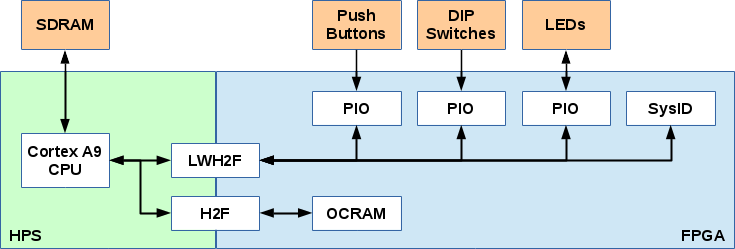
\includegraphics[scale=0.90]{hps_block_diagram}
\caption{HPS System Block Diagram}
\label{fig:hps_block_diagram}
\end{figure}

In this tutorial we will demonstrate how you can interact with the Qsys system in the FPGA through the HPS-to-FPGA bridges provided on the HPS core, reading and writing to the slave peripherals they are connected to.  Both U-Boot console commands and a U-Boot standalone application are used to interact with the soft IP peripherals residing in the FPGA fabric.
\newline
\newline
The following reference materials provide more information about the U-Boot features that are demonstrated in this tutorial:

\begin{itemize}
\item U-Boot Command Line Interface: \href{https://www.denx.de/wiki/view/DULG/UBootCommandLineInterface}{https://www.denx.de/wiki/view/DULG/UBootCommandLineInterface}
\item U-Boot Command Line Parsing: \href{https://www.denx.de/wiki/view/DULG/CommandLineParsing}{https://www.denx.de/wiki/view/DULG/CommandLineParsing}
\item U-Boot Scripting Capabilities: \href{https://www.denx.de/wiki/DULG/UBootScripts}{https://www.denx.de/wiki/DULG/UBootScripts}
\item U-Boot Standalone Applications: \href{https://www.denx.de/wiki/view/DULG/UBootStandalone}{https://www.denx.de/wiki/view/DULG/UBootStandalone}
\end{itemize}

\end{flushleft}

%----NEW SECTION DEFINITION-----------------------------------------------------
\section*{Prerequisites}
% must manually add TOC reference for unnumbered section
\addcontentsline{toc}{section}{Prerequisites}
%----NEW SECTION DEFINITION-----------------------------------------------------

\begin{flushleft}
\noindent
The following are required:

\begin{itemize}

\item Linux\textsuperscript{*} development host PC with internet connection and serial terminal emulator
\item Completed Intel\textsuperscript{\textregistered} Quartus\textsuperscript{\textregistered} software project from \textquote{My First HPS System}
\begin{itemize}
\item Either follow the tutorial steps presented \href{\TheReleasesURL/writeup_MyFirstHPSSystem.pdf}{\underline{here}}.
\item Or, obtain the prebuilt output required from that tutorial \hyperlink{blinkArchive}{\underline{here}}.
\end{itemize}
\item Terasic DE10-Nano SD Card Image Archive: \small \MySDIMAGETGZ \normalsize
\begin{itemize}
\item You can download the archive from this location \href{https://downloadcenter.intel.com/download/26687/Downloads-for-the-Terasic-DE10-Nano-Kit-Featuring-an-Intel-Cyclone-V-FPGA-SoC}{https://\allowbreak downloadcenter.\allowbreak intel.\allowbreak com/\allowbreak download/\allowbreak 26687/\allowbreak Downloads-\allowbreak for-\allowbreak the-\allowbreak Terasic-\allowbreak DE10-\allowbreak Nano-\allowbreak Kit-\allowbreak Featuring-\allowbreak an-\allowbreak Intel-\allowbreak Cyclone-\allowbreak V-\allowbreak FPGA-\allowbreak SoC}
\end{itemize}
\item Terasic DE10-Nano Sources Archive: \small \MySDSRCTGZ \normalsize
\begin{itemize}
\item You can download the archive from this location \href{https://downloadcenter.intel.com/download/26687/Downloads-for-the-Terasic-DE10-Nano-Kit-Featuring-an-Intel-Cyclone-V-FPGA-SoC}{https://\allowbreak downloadcenter.\allowbreak intel.\allowbreak com/\allowbreak download/\allowbreak 26687/\allowbreak Downloads-\allowbreak for-\allowbreak the-\allowbreak Terasic-\allowbreak DE10-\allowbreak Nano-\allowbreak Kit-\allowbreak Featuring-\allowbreak an-\allowbreak Intel-\allowbreak Cyclone-\allowbreak V-\allowbreak FPGA-\allowbreak SoC}
\end{itemize}
\item Terasic DE10-Nano board
\item MicroSD\textsuperscript{*} card for Terasic DE10-Nano
\item MicroSD card adapter for host PC if necessary
\item Power supply for Terasic DE10-Nano
\item Mini USB cable to connect Terasic DE10-Nano UART console port with PC

\end{itemize}

Notes:

\begin{itemize}

\item The SD card image archive, source archive, and the \textbf{blink} hardware project from the \textquote{My First HPS System} tutorial are assumed to be stored in the \textbf{\$DE10\_NANO} folder on the host PC. Make sure you define this environment variable to point at the location where these files are stored. For instance, if you store these files in your \textbf{HOME} directory, in a directory called \textbf{de10-nano}, you can define the environment variable like this:

\begin{minted}[
	bgcolor=MyMintedBGColor,
	escapeinside=++
]{text}

+\$+ export DE10_NANO=+\textasciitilde+/de10-nano

\end{minted}

\item The following files from the \textbf{blink} hardware project are used by this guide:

\begin{itemize}

\item \texttt{blink/output\_files/blink.rbf} - for configuring the FPGA from U-Boot

\item \texttt{blink/qsys\_headers/hps\_0\_arm\_a9\_0.h} - for details about IP addresses inside the FPGA fabric

\end{itemize}

\item \hypertarget{blinkArchive}{If} you need the prebuilt files from the \textbf{blink} hardware project, you can download them to your local file system \href{\TheReleasesURL/blink_for_uboot.zip}{\underline{here}}.  Save the ZIP archive file to this location, \textbf{\$DE10\_NANO/}, the location stored in the environment variable suggested in the note above.  After you have stored the archive you can extract the contents like this:

%\item \hypertarget{blinkArchive}{If} you need the prebuilt files from the \textbf{blink} hardware project, %you can extract this PDF attachment to your local file system: \textattachfile[
%	color=0.0 0.678 0.937,
%	mimetype=application/zip,
%	description={ZIP Archvie File: blink.zip}
%]{../blink_archive/blink.zip}{\textbf{blink.zip}}. Right click on the PDF attachment link and your PDF reader should present a pop-up menu with an option to save the attachment to your local file system.  Save the ZIP archive file to this location, \textbf{\$DE10\_NANO/}, the location stored in the environment variable suggested in the note above.  After you have stored the archive you can extract the contents like this:

\begin{minted}[
	bgcolor=MyMintedBGColor,
	escapeinside=++
]{text}

+\$+ cd +\$+DE10_NANO
+\$+ unzip blink_for_uboot.zip

\end{minted}

\item Throughout this guide, filenames and parameters that can change based on the latest release filenames or host computer configuration are marked in \textcolor{red}{red}.  You may need to change those values based on your specific environment and the version that you are using.

\end{itemize}

\end{flushleft}

%----NEW SECTION DEFINITION-----------------------------------------------------
\section*{Preparing the Terasic DE10-Nano Board}
% must manually add TOC reference for unnumbered section
\addcontentsline{toc}{section}{Preparing the Terasic DE10-Nano Board}
%----NEW SECTION DEFINITION-----------------------------------------------------

\begin{flushleft}
\noindent

This section describes how to prepare the Terasic DE10-Nano board for use in this tutorial.

\begin{enumerate}[
	label=\textbf{Step \arabic*.},
	leftmargin=*,
	widest={00},
	align=left]

\item Remove the microSD card from your Terasic DE10-Nano board and insert it into your host PC using an appropriate adapter if necessary.

\item Extract the SD card image from the archive by running the following command:

\begin{minted}[
	bgcolor=MyMintedBGColor,
	escapeinside=++
]{text}

+\$+ cd +\$+DE10_NANO
+\$+ tar xf +\MySDIMAGETGZ+

\end{minted}

\item Write the SD card image to the microSD card using the \textbf{dd} command:

\begin{minted}[
	bgcolor=MyMintedBGColor,
	escapeinside=++
]{text}

+\$+ sudo dd if=+\MySDIMAGE+ of=+\textcolor{red}{/dev/sdx}+ bs=16M

\end{minted}

After the SD image is copied to your microSD card some systems may automatically detect the new partitions that have been copied onto the microSD card and you will not have to manually probe them.  If you do need to manually probe the partitions to get them to appear in your environment properly, you can do it like this:

\begin{minted}[
	bgcolor=MyMintedBGColor,
	escapeinside=++
]{text}

+\$+ sudo partprobe +\textcolor{red}{/dev/sdx}+

\end{minted}

\item Mount the FAT partition of the microSD card on the host PC, and copy the \textbf{blink.rbf} FPGA configuration file to it. Depending on your host PC configuration, the mounting may happen automatically. The FAT partition is partition 1 on the microSD card.  The instructions below assume manual mounting is needed:

\begin{minted}[
	bgcolor=MyMintedBGColor,
	escapeinside=++
]{text}

# create a directory in +\$+DE10_NANO to use as a mount point
+\$+ mkdir sdcard

# mount partition 1 of the microSD card, this is the FAT partition
+\$+ sudo mount +\textcolor{red}{/dev/sdx}+1 sdcard

# copy the required file onto the FAT partition
+\$+ sudo cp +\$+DE10_NANO/blink/output_files/blink.rbf sdcard/

# unmount the FAT partition
+\$+ sudo umount sdcard
+\$+ sudo sync

\end{minted}

\item Remove the microSD card from your host PC and insert it into the Terasic DE10-Nano board.

\newpage

\item Configure the Terasic DE10-Nano dip switch block \textbf{SW10} (highlighted in red below) to these positions from left to right as viewed with the board oriented as shown in the image below: \texttt{UP-DOWN-UP-DOWN-UP-UP}

\begin{figure}[H]
\centering
% screen shots report a density of 37.8 PixelsPerCentimeter when actual resolution
% is more like 56 PixelsPerCentimeter, so the scaling factor for 1:1 is 0.675
\scriptsize{Image used with permission from Terasic Technologies Inc.}
\newline
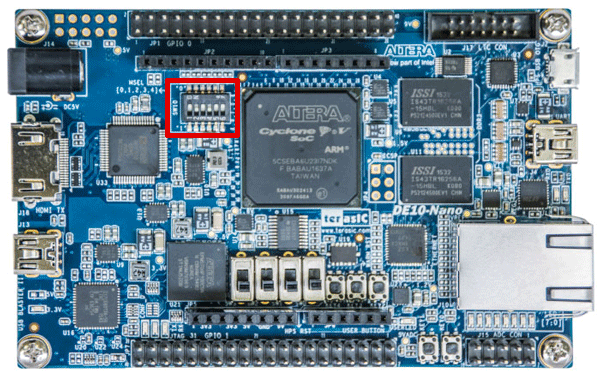
\includegraphics[scale=0.675]{de10-nano_sw10}
\caption{SW10 Configuration}
\label{fig:de10-nano_sw10}
\end{figure}

\item Plug a mini USB cable into the Terasic DE10-Nano UART console connector (highlighted in red below),  then plug the other end of the USB cable into your host PC.

\begin{figure}[H]
\centering
% screen shots report a density of 37.8 PixelsPerCentimeter when actual resolution
% is more like 56 PixelsPerCentimeter, so the scaling factor for 1:1 is 0.675
\scriptsize{Image used with permission from Terasic Technologies Inc.}
\newline
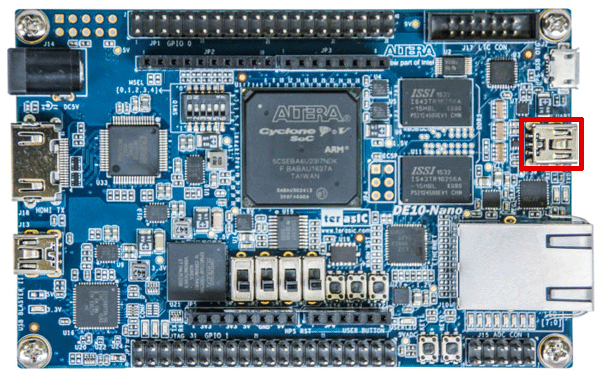
\includegraphics[scale=0.675]{de10-nano_uart}
\caption{UART Console Connector on Terasic DE10-Nano Board}
\label{fig:de10-nano_uart}
\end{figure}

\newpage

\item On the host PC, start a serial terminal (for example minicom, or putty) and connect to the serial port corresponding to the Terasic DE10-Nano UART console using the serial communication settings: \texttt{115,200-8-N-1}.

\item \textcolor{red}{\emph{Read the next step before completing this step.}} Power the Terasic DE10-Nano board by inserting the power supply cord into the power connector (highlighted in red below).

\begin{figure}[H]
\centering
% screen shots report a density of 37.8 PixelsPerCentimeter when actual resolution
% is more like 56 PixelsPerCentimeter, so the scaling factor for 1:1 is 0.675
\scriptsize{Image used with permission from Terasic Technologies Inc.}
\newline
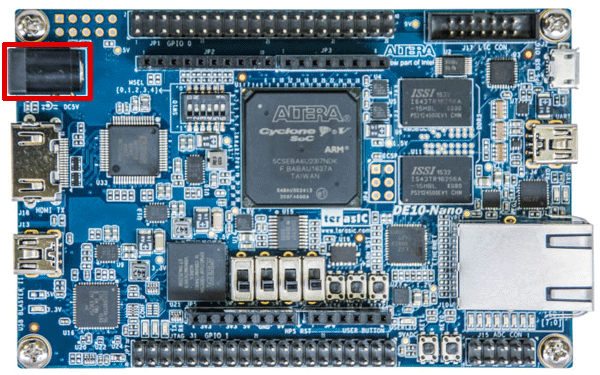
\includegraphics[scale=0.675]{de10-nano_pwr}
\caption{Power Connector on Terasic DE10-Nano Board}
\label{fig:de10-nano_pwr}
\end{figure}

\item In the serial terminal, interrupt the U-Boot autoboot countdown by pressing any key. This will provide access to the U-Boot console.  If you are too slow and the Linux kernel begins to boot, you should allow Linux to load, login with the username \textbf{root} and empty password (simply press the \textbf{enter} key for the password).  Then run the Linux command \textbf{reboot} which will shutdown the Linux session and reboot through U-Boot.  Try to be quicker on the next pass through U-Boot and stop it by pressing any key during the autoboot countdown.  Repeat as necessary.

\begin{minted}[
	bgcolor=MyMintedBGColor,
	escapeinside=++
]{text}

U-Boot SPL 2017.03-rc2 (Mar 30 2017 - 19:07:16)
/data/de10-nano/release-build-2017.03.31/build/tmp-angstrom-glibc/work/de10_nano
-angstrom-linux-gnueabi/u-boot-socfpga/v2017.03+gitAUTOINC+d03450606b-r0/git/dri
vers/ddr/altera/sequencer.c: Preparing to start memory calibration
/data/de10-nano/release-build-2017.03.31/build/tmp-angstrom-glibc/work/de10_nano
-angstrom-linux-gnueabi/u-boot-socfpga/v2017.03+gitAUTOINC+d03450606b-r0/git/dri
vers/ddr/altera/sequencer.c: CALIBRATION PASSED
/data/de10-nano/release-build-2017.03.31/build/tmp-angstrom-glibc/work/de10_nano
-angstrom-linux-gnueabi/u-boot-socfpga/v2017.03+gitAUTOINC+d03450606b-r0/git/dri
vers/ddr/altera/sequencer.c: Calibration complete
Trying to boot from MMC1


U-Boot 2017.03-rc2 (Mar 30 2017 - 19:07:16 -0700)

CPU:   Altera SoCFPGA Platform
FPGA:  Altera Cyclone V, SE/A6 or SX/C6 or ST/D6, version 0x0
BOOT:  SD/MMC Internal Transceiver (3.0V)
       Watchdog enabled
I2C:   ready
DRAM:  1 GiB
MMC:   dwmmc0@ff704000: 0
*** Warning - bad CRC, using default environment

In:    serial
Out:   serial
Err:   serial
Model: Terasic DE10-Nano
Net:
Error: ethernet@ff702000 address not set.
No ethernet found.
Hit any key to stop autoboot:  0
=>

\end{minted}

\item On the U-Boot console, run the following commands to configure the FPGA with the \textbf{blink.rbf} file from the SD card

\begin{minted}[
	bgcolor=MyMintedBGColor,
	escapeinside=++
]{text}

=> load mmc 0:1 +\$+{kernel_addr_r} blink.rbf
=> fpga load 0 +\$+{kernel_addr_r} +\$+{filesize}
=> bridge enable

\end{minted}

You should see the amber \textbf{conf\_done} LED illuminate once the commands above complete.

\end{enumerate}

\end{flushleft}

%----NEW SECTION DEFINITION-----------------------------------------------------
\section*{Using U-Boot Commands to Interact with the FPGA Design}
% must manually add TOC reference for unnumbered section
\addcontentsline{toc}{section}{Using U-Boot Commands to Interact with the FPGA Design}
%----NEW SECTION DEFINITION-----------------------------------------------------

\begin{flushleft}
\noindent

This section describes various U-Boot commands and techniques for interacting with the FPGA design.

\begin{enumerate}[
	label=\textbf{Step \arabic*.},
	leftmargin=*,
	widest={00},
	align=left]

\item Boot into the U-Boot console, and configure FPGA with the \textbf{blink.rbf} as described in the \textquote{Preparing the Terasic DE10-Nano Board} section above.

\item Next, we will interact with the IP modules inside the FPGA fabric. This will require us to recall the address map produced in the previous tutorial.  Remember that we used the \textbf{sopc-create-header-files} in that tutorial to create the \textbf{hps\_0\_arm\_a9\_0.h} header file, and then we dumped all of the base address macros from that file.  To refresh your memory, here is what those addresses are:

\begin{minted}[
        bgcolor=MyMintedBGColor,
        escapeinside=++
]{c}

#define OCRAM_64K_BASE 0x0
#define LED_PIO_BASE 0x10000
#define BUTTON_PIO_BASE 0x10010
#define SWITCH_PIO_BASE 0x10020
#define SYSTEM_ID_BASE 0x10030

\end{minted}

We will set a number of U-Boot variables to allow us to recall these base addresses easier in the rest of this tutorial.  Execute these commands on the U-Boot console to setup these variables:

\begin{minted}[
	bgcolor=MyMintedBGColor,
	escapeinside=++
]{text}

=> OCRAM_64K_BASE=0xc0000000
=> LED_PIO_BASE=0xff210000
=> BUTTON_PIO_BASE=0xff210010
=> SWITCH_PIO_BASE=0xff210020
=> SYSTEM_ID_BASE=0xff210030

\end{minted}

\newpage

\item Exercise the IP inside the FPGA fabric by running various commands

\begin{enumerate}[
	label=\textbf{Step \arabic{enumi}\alph*.},
	leftmargin=*,
	align=left]

\item Interact with the onchip RAM component.

\begin{minted}[
	bgcolor=MyMintedBGColor,
	escapeinside=++
]{text}

# read the onchip RAM
=> md.l +\$+OCRAM_64K_BASE 1
c0000000: 00000000                               ....

# write a pattern to the onchip RAM
=> mw.l +\$+OCRAM_64K_BASE 0x1234de10

# verify the pattern remains in the onchip RAM
=> md.l +\$+OCRAM_64K_BASE 1
c0000000: 1234de10                               ..4.

\end{minted}

\item Interact with the LED PIO component.

\begin{minted}[
	bgcolor=MyMintedBGColor,
	escapeinside=||
]{text}

# turn on half the LEDs
=> mw.l |\$|LED_PIO_BASE 0x55

# turn off those LEDs and turn on the other half of the LEDs
=> mw.l |\$|LED_PIO_BASE 0xaa

# write a loop to toggle LED0 and LED1 every half second for 10 times
=> setenv COUNT 0
=> while itest |\$|{COUNT} < 0x0a
> do
> mw.l |\$|LED_PIO_BASE 0x01
> sleep 0.5
> mw.l |\$|LED_PIO_BASE 0x02
> sleep 0.5
> setexpr COUNT |\$|{COUNT} + 1
> done

# turn on all of the LEDs
=> mw.l |\$|LED_PIO_BASE 0xff

\end{minted}

\item Exercise the HPS-to-FPGA reset functionality.  Now that we have some LEDs illuminated, let's look at how the HPS-to-FPGA reset can be triggered.  We have the ability to assert the reset provided into the FPGA by the HPS core, to do that we use the following commands to set and clear the \textbf{s2f} bit of the \textbf{miscmodrst} register located in the HPS Reset Manager, that is bit 6 of the HPS register at address 0xFFD05020:

\begin{minted}[
	bgcolor=MyMintedBGColor,
	escapeinside=++
]{text}

# assert the H2F reset
=> mw.l 0xFFD05020 0x40

# deassert the H2F reset
=> mw.l 0xFFD05020 0x00

\end{minted}

After executing the first command, the LEDs should all turn off, returned to their reset state.  Do not forget to release the reset by clearing that bit with the second command.  You can trigger the same reset effect by pressing the KEY0 push button.  Turn on some LEDs again and try pressing KEY0 to prove that as well.
\newline
\newline
Please note that resetting the FPGA logic design while software is running on the HPS core can be dangerous for the software environment.  If software drivers are interacting with FPGA logic at the time you invoke a reset like this, the hardware transactions can hang which causes the software environment to hang.  So resetting part of the hardware system like this should be done with caution.

\item Interact with the button PIO component.  The KEY1 push button is connected to this PIO peripheral.

\begin{minted}[
	bgcolor=MyMintedBGColor,
	escapeinside=++
]{text}

# read the button with KEY1 not pressed
=> md.l +\$+BUTTON_PIO_BASE 1
ff210010: 00000001                               ....

# read the button with KEY1 pressed
=> md.l +\$+BUTTON_PIO_BASE 1
ff210010: 00000000                               ....

# read the button with KEY1 not pressed
=> md.l +\$+BUTTON_PIO_BASE 1
ff210010: 00000001                               ....

\end{minted}

\item Interact with the switch PIO component.  The four slide switches are connected to this PIO peripheral.

\begin{minted}[
	bgcolor=MyMintedBGColor,
	escapeinside=++
]{text}

# all switches in the up position
=> md.l +\$+SWITCH_PIO_BASE 1
ff210020: 0000000f                               ....

# far right switch moved down
=> md.l +\$+SWITCH_PIO_BASE 1
ff210020: 0000000e                               ....

# next switch to the left moved down
=> md.l +\$+SWITCH_PIO_BASE 1
ff210020: 0000000c                               ....

# next switch to the left moved down
=> md.l +\$+SWITCH_PIO_BASE 1
ff210020: 00000008                               ....

# last switch moved down
=> md.l +\$+SWITCH_PIO_BASE 1
ff210020: 00000000                               ....

\end{minted}

\item Interact with the system ID component.  This component contains two 32-bit words, one ID value that we set to the value 0xde10de10 in the previous hardware portion of this tutorial and the second word that represents the unix second time value when the Qsys system was generated.

\begin{minted}[
	bgcolor=MyMintedBGColor,
	escapeinside=++
]{text}

=> md.l +\$+SYSTEM_ID_BASE 2
ff210030: de10de10 59187c42                      ....B|.Y

\end{minted}

\item Exercise the default slave peripheral.  Here we will demonstrate what happens when we read and write to unmapped address spans.

\begin{minted}[
	fontsize=\small,
	bgcolor=MyMintedBGColor,
	escapeinside=++
]{text}

# our peripherals are mapped into the HPS address span through the LWHPS bridge
# from 0xFF21_0000 thru 0xFF21_0038 and the HPS bridge from 0xC000_0000 thru
# 0xC000_FFFF, so we choose an arbitrary high address well above our peripherals
# and we read the 16 bytes of the default slave peripheral which should be
# initialized at device configuration to 0x0000_0000
=> md.l 0xff211000 4
ff211000: 00000000 00000000 00000000 00000000    ................

# now lets set those 4 words with a specific incrementing pattern
=> mw.l 0xff211000 0x0badf00d
=> mw.l 0xff211004 0x1badf00d
=> mw.l 0xff211008 0x2badf00d
=> mw.l 0xff21100c 0x3badf00d

# now validate that pattern repeats every 4 words
=> md.l 0xff211000 8
ff211000: 0badf00d 1badf00d 2badf00d 3badf00d    ...........+...;
ff211010: 0badf00d 1badf00d 2badf00d 3badf00d    ...........+...;

# now lets write to a slave that has no write interface, like the system ID
# peripheral.  That write will not be decoded by any slave in the system and
# will be directed into the default slave
=> mw.l +\$+SYSTEM_ID_BASE 0xfacecafe

# now verify that the first word of the default slave was actually written
=> md.l 0xff211000 4
ff211000: facecafe 1badf00d 2badf00d 3badf00d    ...........+...;

# we have been using an address in the LWHPS bridge address span, but we can see
# the default slave through the HPS bridge as well
=> md.l 0xc0010000 4
c0010000: facecafe 1badf00d 2badf00d 3badf00d    ...........+...;

\end{minted}

\end{enumerate}

\end{enumerate}

That's it, you've interacted with the Qsys system using U-Boot commands.  Continue on to the next section where we demonstrate how to write a standalone U-Boot program to interact with the Qsys system.

\end{flushleft}

%----NEW SECTION DEFINITION-----------------------------------------------------
\section*{Using U-Boot Applications to Interact with the FPGA Design}
% must manually add TOC reference for unnumbered section
\addcontentsline{toc}{section}{Using U-Boot Applications to Interact with the FPGA Design}
%----NEW SECTION DEFINITION-----------------------------------------------------

\begin{flushleft}
\noindent

This section presents the following:

\begin{itemize}

\item Getting the required cross compiler toolchain and the U-Boot sources

\item Writing a U-Boot application that exercises the IP inside the FPGA fabric

\item Compiling the U-Boot application

\item Running the U-Boot application

\end{itemize}

\begin{enumerate}[
	label=\textbf{Step \arabic*.},
	leftmargin=*,
	widest={00},
	align=left]

\item Save the sources archive \MySDSRCTGZ \ to the \textbf{\$DE10\_NANO} directory on the host PC.

\item Run the following commands to get the toolchain, and prepare the U-Boot sources:

\begin{minted}[
	bgcolor=MyMintedBGColor,
	escapeinside=++
]{text}

# change into the tutorial directory
+\$+ cd +\$+DE10_NANO

# get the linaro ARM GCC toolchain
+\$+ wget https://releases.linaro.org/components/toolchain/binaries/6.2-2016.11/\
> arm-linux-gnueabihf/gcc-linaro-6.2.1-2016.11-x86_64_arm-linux-gnueabihf.tar.xz

# extract the toolchain
+\$+ tar xf gcc-linaro-6.2.1-2016.11-x86_64_arm-linux-gnueabihf.tar.xz

# extract the sources archive
+\$+ tar xf +\MySDSRCTGZ+

# retrieve the U-Boot archives from the extracted sources archive
+\$+ cp -r sources/arm-angstrom-linux-gnueabi/u-boot-socfpga* uboot-socfpga

# extract the U-Boot archives
+\$+ cd uboot-socfpga
+\$+ tar xf u-boot-socfpga-*-r0.tar.gz
+\$+ tar xf u-boot-socfpga-*-r0-hardware.tar.gz

# patch the U-Boot sources with the DE10-Nano changes
+\$+ cd git
+\$+ cat ../*.patch | patch -p1

\end{minted}

The U-Boot standalone application examples are stored in \textbf{\$DE10\_NANO/\allowbreak uboot-socfpga/\allowbreak git/\allowbreak examples/\allowbreak standalone/}.

\item Copy the \textbf{blink/qsys\_headers/hps\_0\_arm\_a9\_0.h} header created in the previous tutorial into the U-Boot standalone examples directory:

\begin{minted}[
	bgcolor=MyMintedBGColor,
	escapeinside=++
]{text}

# copy hps_0_arm_a9_0.h into u-boot standalone examples directory
+\$+ cp +\$+DE10_NANO/blink/qsys_headers/hps_0_arm_a9_0.h \
> +\$+DE10_NANO/uboot-socfpga/git/examples/standalone/

\end{minted}

%\item Extract this PDF attachment to your local file system: \textattachfile[
%	color=0.0 0.678 0.937,
%	mimetype=text/plain,
%	description={C Source File: blink\_app.c}
%]{../c_examples/blink_app.c}{\textbf{blink\_app.c}}.  Right click on the PDF attachment link and your PDF reader should present a pop-up menu with an option to save the attachment to your local file system.  Save the C source file to this location \textbf{\$DE10\_NANO/\allowbreak uboot-socfpga/\allowbreak git/\allowbreak examples/\allowbreak standalone/\allowbreak blink\_app.c}.  These are the contents of the standalone application:

\item Download the blink\_app.c file \href{\TheRawURL/MyFirstHPSSystem/writeup_u-boot/c_examples/blink_app.c}{\underline{here}}.  Save the C source file to this location \textbf{\$DE10\_NANO/\allowbreak uboot-socfpga/\allowbreak git/\allowbreak examples/\allowbreak standalone/\allowbreak blink\_app.c}.  If you wish to view the blink\_app.c file in the GitHub\textsuperscript{*} repo you can look \href{\TheBlobURL/MyFirstHPSSystem/writeup_u-boot/c_examples/blink_app.c}{\underline{here}}.  These are the contents of the standalone application:


\inputminted[
	bgcolor=MyMintedBGColor,
	linenos,
	fontsize=\normalsize
]{c}{../c_examples/blink_app.c}

\item Edit the file \textbf{\$DE10\_NANO/\allowbreak uboot-socfpga/\allowbreak git/\allowbreak examples/\allowbreak standalone/\allowbreak Makefile} to add the \textbf{blink\_app} to the list of applications to be compiled, by adding the line highlighted below:

\begin{minted}[
	bgcolor=MyMintedBGColor,
	escapeinside=||
]{text}

extra-y        := hello_world
|\hl{extra}\hl{\textminus}\hl{y}\hl{        +=}\hl{ blink\_app}|
extra-y        += de10_nano_hdmi_config

\end{minted}

You can do this by opening the Makefile in a text editor, or you can apply the update using \textbf{sed} like this:

\begin{minted}[
	bgcolor=MyMintedBGColor,
	escapeinside=||
]{text}

|\$| sed -i.bak -e "/.*hello_world/a extra-y\ \ \ \ \ \ \ \ += blink_app" \
> |\$|DE10_NANO/uboot-socfpga/git/examples/standalone/Makefile

\end{minted}

\item Compile the U-Boot applications by running the commands below:

\begin{minted}[
	fontsize=\small,
	bgcolor=MyMintedBGColor,
	escapeinside=++
]{text}

# change into the U-Boot top level source directory
+\$+ cd +\$+DE10_NANO/uboot-socfpga/git

# configure the CROSS_COMPILE environment variable to use the toolchain that
# we previously downloaded
+\$+ export CROSS_COMPILE=+\$+DE10_NANO/gcc-linaro-6.2.1-2016.11-x86_64_arm-linux-gnueabihf/
+\$+ export CROSS_COMPILE=+\$+{CROSS_COMPILE}bin/arm-linux-gnueabihf-

# build the U-Boot standalone examples
+\$+ make socfpga_de10_nano_defconfig
+\$+ make examples

\end{minted}

This will build all the examples, including the \textbf{blink\_app} we added, which will be accessible at \textbf{\$DE10\_NANO/\allowbreak uboot-socfpga/\allowbreak git/\allowbreak examples/\allowbreak standalone/\allowbreak blink\_app.bin}.

\item Use the microSD card created in the \textquote{Preparing the Terasic DE10-Nano Board} section above and copy the \textbf{blink\_app.bin} file to it the way we copied the \textbf{blink.rbf} file.  The instructions below assume manual mounting is needed:

\begin{minted}[
	bgcolor=MyMintedBGColor,
	escapeinside=++
]{text}

+\$+ cd +\$+DE10_NANO
+\$+ mkdir sdcard
+\$+ sudo mount +\textcolor{red}{/dev/sdx}+1 sdcard
+\$+ sudo cp +\$+DE10_NANO/uboot-socfpga/git/examples/standalone/blink_app.bin sdcard/
+\$+ sudo umount +\textcolor{red}{/dev/sdx}+1
+\$+ sudo sync

\end{minted}

\item Boot into the U-Boot console, and configure the FPGA with the \textbf{blink.rbf} file as described in the \textquote{Preparing the Terasic DE10-Nano Board} section above.

\item Load and execute the \textbf{blink\_app} from the U-Boot console:

\begin{minted}[
	bgcolor=MyMintedBGColor,
	escapeinside=++
]{text}

=> load mmc 0:1 0x0c100000 blink_app.bin
=> go 0x0C100001 hello world

\end{minted}

\item Interact with the application as instructed on the U-Boot console:

\begin{minted}[
	bgcolor=MyMintedBGColor,
	escapeinside=++
]{text}

## Starting application at 0x0C100001 ...

Blink application started.

Number of command line parameters: 3
Command line parameter 1 = 0x0C100001
Command line parameter 2 = hello
Command line parameter 3 = world

U-Boot ABI version 9

SysID.id = 0xde10de10
SysID.timestamp = 0x5931e56f

Writing pattern into FPGA OCRAM.
Checking pattern from FPGA OCRAM: passed.

Blinking LEDs
Press any key to stop LED lightshow

Displaying the state of switches
Slide switch SW0, Sw1, SW2 or SW3 to observe updates
Press any key to stop displaying the switches
Switch value: 0xf
Switch value: 0xe
Switch value: 0xc
Switch value: 0x8
Switch value: 0x0

Displaying the state of buttons
Press push button KEY1 to observe updates
Press any key to stop displaying the buttons
Button value: 0x1
Button value: 0x0
Button value: 0x1
Button value: 0x0
Button value: 0x1

Blink Application completed.

## Application terminated, rc = 0x0
=>

\end{minted}

\end{enumerate}

That's it, you've interacted with the Qsys system using a custom standalone U-Boot application.  Continue on to the \textquote{Interacting with FPGA Designs using Linux} tutorial if you would like to see how to do similar things from a Linux environment running on the HPS processor.

\end{flushleft}

\end{document}

